\documentclass[11pt]{article}

% ---------- Page / fonts ----------
\usepackage[letterpaper,margin=1in]{geometry}
\usepackage[T1]{fontenc}
\usepackage{amsmath,amssymb,amsthm}
\usepackage{graphicx}
\usepackage{xcolor}
\usepackage{booktabs}
\usepackage{tcolorbox}
\usepackage{enumitem}
\usepackage{fancyhdr}
\usepackage{listings}
\usepackage{tikz}
\usetikzlibrary{shapes,arrows.meta,positioning,calc}
\usepackage{placeins}
\usepackage{float}
\usepackage[colorlinks=true,linkcolor=accent,urlcolor=accent]{hyperref}

% ---------- Identity / colours ----------
\definecolor{accent}{HTML}{1F4E79}
\definecolor{soft}{HTML}{F4F7FB}
\definecolor{rule}{HTML}{C9D6E5}

\newcommand{\name}{Kaushik Vada}
\newcommand{\course}{EE 132 --- Automatic Control}
\newcommand{\hwnum}{Homework 6}
\newcommand{\hwsub}{Lead \& Lag Compensator Design}

% ---------- Header / footer ----------
\pagestyle{fancy}
\fancyhf{}
\setlength{\headheight}{14pt}
\renewcommand{\headrulewidth}{0.4pt}
\renewcommand{\footrulewidth}{0pt}
\lhead{\small\textcolor{accent}{\textbf{\course}}}
\rhead{\small\textcolor{accent}{\hwnum}}
\cfoot{\small\thepage}

% ---------- Solution box ----------
\newtcolorbox{solution}{
  colback=soft, colframe=accent,
  boxrule=0.6pt, left=10pt, right=10pt, top=8pt, bottom=8pt,
  arc=2pt,
  title=\textbf{Solution}, fonttitle=\color{white}\bfseries, coltitle=white
}

% ---------- Problem heading ----------
\newcommand{\problem}[2]{%
  \vspace{4pt}
  \noindent{\large\textbf{\textcolor{accent}{Problem #1.}}\ \ #2}\par
  \vspace{2pt}\noindent\textcolor{rule}{\rule{\linewidth}{0.8pt}}\par\vspace{4pt}
}

% ---------- MATLAB listing style ----------
\lstdefinestyle{matlab}{
  language=Matlab,
  basicstyle=\ttfamily\footnotesize,
  keywordstyle=\color{accent}\bfseries,
  commentstyle=\color{gray}\itshape,
  stringstyle=\color{teal},
  numbers=left, numberstyle=\tiny\color{gray}, numbersep=8pt,
  frame=single, rulecolor=\color{rule},
  backgroundcolor=\color{soft},
  breaklines=true, showstringspaces=false,
  xleftmargin=14pt, framexleftmargin=12pt,
  aboveskip=8pt, belowskip=4pt
}

\setlist[enumerate]{leftmargin=2.2em}
\newcommand{\dd}{\mathrm{d}}

\begin{document}

% ================= Title =================
\begin{center}
  {\LARGE\bfseries\textcolor{accent}{\course}}\\[4pt]
  {\Large\hwnum\,: \hwsub}\\[8pt]
  {\large\name}\\[2pt]
  \textcolor{rule}{\rule{0.5\linewidth}{0.6pt}}
\end{center}
\vspace{6pt}

\noindent
All three problems use the unity-feedback configuration of Fig.~\ref{fig:loop}, with plant
$G(s)$ and series compensator $D(s)$. Designs are carried out on the root locus (angle and
magnitude conditions) and verified numerically; equivalent MATLAB code is listed with each
solution.

\begin{figure}[htbp]
\centering
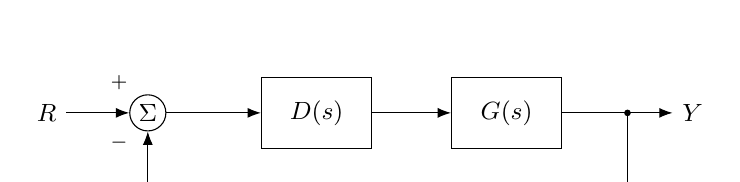
\begin{tikzpicture}[>=Latex, node distance=14mm, font=\small]
  \node (R) {$R$};
  \node[draw,circle,inner sep=1.4pt,right=8mm of R] (sum) {$\Sigma$};
  \node[draw,minimum width=14mm,minimum height=9mm,right=12mm of sum] (D) {$D(s)$};
  \node[draw,minimum width=14mm,minimum height=9mm,right=10mm of D] (G) {$G(s)$};
  \node[right=14mm of G] (Y) {$Y$};
  \coordinate (tap) at ($(G.east)!0.5!(Y)$);
  \draw[->] (R) -- (sum);
  \draw[->] (sum) -- (D);
  \draw[->] (D) -- (G);
  \draw[->] (G) -- (Y);
  \node[above left=0pt and -1pt of sum] {\scriptsize $+$};
  \node[below left=0pt and -1pt of sum] {\scriptsize $-$};
  \draw[->] (tap) -- ++(0,-10mm) -| (sum);
  \fill (tap) circle (1.2pt);
\end{tikzpicture}
\caption{Unity-feedback configuration (Fig.~5.60).}
\label{fig:loop}
\end{figure}

% ====================================================================
\problem{26}{Numerically controlled machine-tool servomechanism}

\noindent The normalized plant is
\[
  G(s)=\frac{1}{s(s+1)},
\]
and the closed-loop poles are to be placed at $s=-1\pm j\sqrt3$
(i.e.\ $\omega_n=2$, $\zeta=\tfrac12$).

\begin{solution}
\textbf{(a) Proportional control is insufficient.}
With $D(s)=k_p$ the loop gain is $L(s)=\dfrac{k_p}{s(s+1)}$ and the characteristic
equation is
\[
  s(s+1)+k_p=0 \;\Longrightarrow\; s^2+s+k_p=0 .
\]
By Vieta's formula the two roots always sum to $-1$, so a complex-conjugate pair has
\[
  \operatorname{Re}(s)=-\tfrac12 \quad\text{for every } k_p .
\]
The target poles require $\operatorname{Re}(s)=-1$, which is unreachable. Equivalently, on
the root locus the angle condition at $s_0=-1+j\sqrt3$ gives
\[
  \angle G(s_0)= -\angle s_0-\angle(s_0+1)
  = -120^\circ-90^\circ=-210^\circ\equiv 150^\circ\neq \pm180^\circ,
\]
so $s_0$ is \emph{not} on the locus. The angle deficiency is
$\phi = 180^\circ-150^\circ = 30^\circ$, which a lead network must supply.

\medskip
\textbf{(b) Lead design $D(s)=K\dfrac{s+z}{s+p}$.}
Cancel the plant pole at $-1$ by placing the zero at $z=1$. The zero then contributes
$\angle(s_0+1)=+90^\circ$, so the pole must supply the remaining
$90^\circ-60^\circ=30^\circ$ net, i.e.\ $\angle(s_0+p)=60^\circ$:
\[
  \tan 60^\circ=\frac{\sqrt3}{\,p-1\,}=\sqrt3 \;\Longrightarrow\; p=2 .
\]
The magnitude condition $|L(s_0)|=1$ with $L(s)=\dfrac{K}{s(s+2)}$ gives
\[
  \frac{K}{|s_0|\,|s_0+2|}=\frac{K}{(2)(2)}=1\;\Longrightarrow\;K=4 .
\]
Hence
\[
  \boxed{\,D(s)=\dfrac{4(s+1)}{s+2}\,},\qquad
  L(s)=\frac{4}{s(s+2)},\qquad s^2+2s+4=0\;\Rightarrow\; s=-1\pm j\sqrt3 .
\]
The poles land \emph{exactly} on the specification. The velocity constant is
$K_v=\lim_{s\to0}sL(s)=4/2=2$, giving a ramp error of $0.5$. Numerical check:
$\zeta=0.5$, $M_p=16.3\%$ (Fig.~\ref{fig:p26step}, \ref{fig:p26rl}).
\end{solution}

\begin{figure}[htbp]
\centering
\begin{minipage}{0.49\linewidth}\centering
  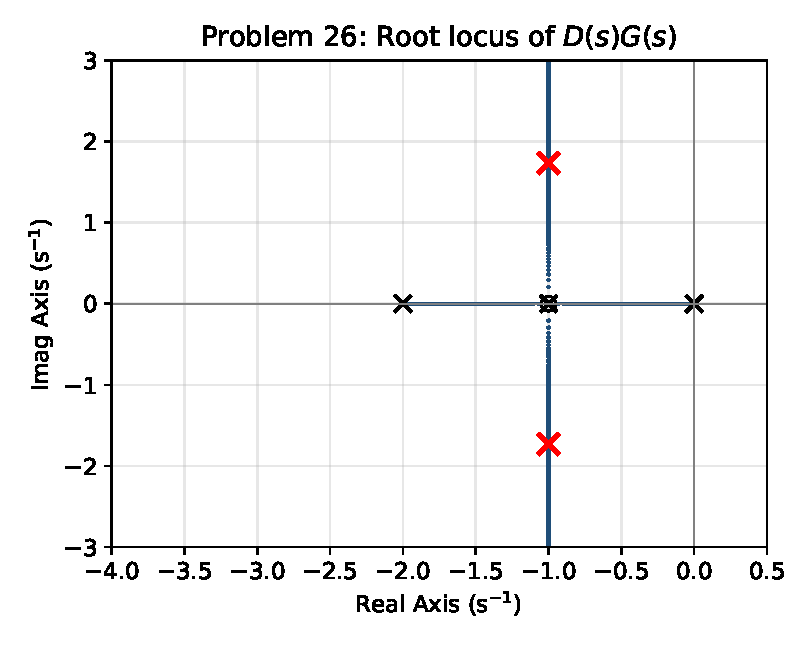
\includegraphics[width=\linewidth]{figures/p26_rlocus.pdf}
  \caption{P26 root locus of $D(s)G(s)$; $\times$ marks the design poles.}
  \label{fig:p26rl}
\end{minipage}\hfill
\begin{minipage}{0.49\linewidth}\centering
  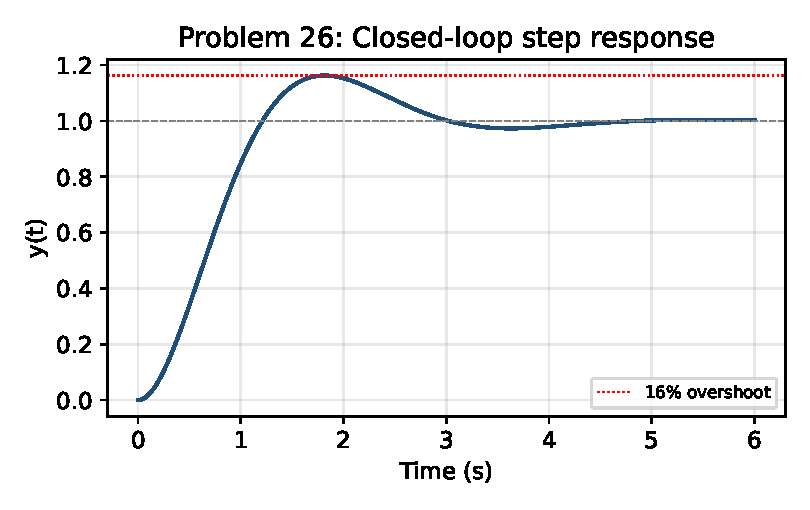
\includegraphics[width=\linewidth]{figures/p26_step.pdf}
  \caption{P26 closed-loop step response.}
  \label{fig:p26step}
\end{minipage}
\end{figure}

\begin{lstlisting}[style=matlab,caption={Problem 26 --- MATLAB}]
s = tf('s');
G = 1/(s*(s+1));
% (b) lead: zero cancels pole at -1, pole at -2, gain K=4
D = 4*(s+1)/(s+2);
L = D*G;  T = feedback(L,1);
damp(T)              % check poles at -1 +/- j*sqrt(3)
Kv = dcgain(s*L)     % velocity constant = 2
figure, rlocus(L),  sgrid(0.5,2)
figure, step(T)
\end{lstlisting}

\FloatBarrier
% ====================================================================
\problem{27}{Servomechanism position control --- lead\,+\,lag}

\noindent
\[
  G(s)=\frac{10}{s(s+1)(s+10)} .
\]
Closed-loop specifications:
\begin{itemize}[nosep,leftmargin=1.6em]
  \item step overshoot $M_p\le 16\% \;\Rightarrow\; \zeta\ge 0.5$;
  \item rise time $t_r\le 0.4\ \text{s} \;\Rightarrow\; \omega_n\ge 1.8/t_r = 4.5\ \text{rad/s}$;
  \item ramp error $e_{ss}<0.02 \;\Rightarrow\; K_v>50$.
\end{itemize}

\begin{solution}
\textbf{Design target.} Because the lead zero raises the actual overshoot above the
second-order estimate, I aim inside the boundary: $\zeta=0.65$, $\omega_n=5.5$, which keeps
$M_p$ comfortably under $16\%$ while giving $\omega_n$ enough for the rise-time spec:
\[
  s_0=-\zeta\omega_n + j\omega_n\sqrt{1-\zeta^2}=-3.58+j4.18 .
\]

\textbf{(a) Lead compensation.} Cancel the plant pole at $-1$ with the lead zero ($z=1$).
The open loop becomes $L(s)=\dfrac{10K}{s(s+10)(s+p)}$. With
$\angle s_0=130.5^\circ$ and $\angle(s_0+10)=33.0^\circ$, the angle condition needs
\[
  \angle(s_0+p)=180^\circ-130.5^\circ-33.0^\circ=16.4^\circ
  \;\Longrightarrow\; p=-\!\operatorname{Re}(s_0)+\frac{\operatorname{Im}(s_0)}{\tan 16.4^\circ}=17.76 .
\]
The magnitude condition $|L(s_0)|=1$, i.e.\ $K=\dfrac{|s_0|\,|s_0+10|\,|s_0+p|}{10}$, gives
$K=62.36$, so
\[
  \boxed{\,D_{\text{lead}}(s)=\dfrac{62.36\,(s+1)}{s+17.76}\,}.
\]
The lead-only closed-loop poles are $-3.55\pm j4.15$ and $-20.6$; the transient specs are met
($M_p\approx7\%$, $t_r\approx0.38$~s), but
$K_v=62.36\cdot\frac{1}{17.76}=3.5$, far short of $50$.

\medskip
\textbf{(b) Proportional control --- velocity constant.}
For $D(s)=k_p$,
\[
  K_v=\lim_{s\to0}s\,k_p\,G(s)=k_p\cdot\frac{10}{(1)(10)}=k_p .
\]
Meeting $K_v>50$ would require $k_p>50$. But $k_p=50$ gives the characteristic polynomial
$s^3+11s^2+10s+500$, whose Routh array has the $s^1$ entry
$\tfrac{11\cdot10-500}{11}=-35.5<0$: \emph{two right-half-plane poles}
($s=0.48\pm j6.84$), i.e.\ the loop is unstable. Proportional control therefore cannot meet
the steady-state requirement while remaining stable --- dynamic (lead\,+\,lag) compensation is
required.

\medskip
\textbf{(c) Lag compensation.} The lag must raise $K_v$ from $3.5$ to above $50$, a factor of
at least $14$; take $\alpha=z/p=25$ for margin and place the dipole near the origin so the
dominant transient is unchanged: $z=0.05$, $p=z/\alpha=0.002$. The complete compensator is
\[
  \boxed{\,D(s)=62.36\,\dfrac{(s+1)(s+0.05)}{(s+17.76)(s+0.002)}\,}.
\]
Then $K_v=3.5\times25\approx88$, so $e_{ss}=1/K_v=0.011<0.02$. Numerical verification of the
final design:
\[
  M_p=7.4\%,\quad t_r=0.38~\text{s},\quad t_s\approx1.2~\text{s},\quad K_v=88,\quad e_{ss}=0.011,
\]
with dominant poles $-3.55\pm j4.15$, a fast pole at $-20.6$, and the lag pole/zero pair near
$-0.05$. All three specifications are satisfied. The root locus and step response of the final
design are shown in Fig.~\ref{fig:p27rl}--\ref{fig:p27step}.
\end{solution}

\begin{figure}[htbp]
\centering
\begin{minipage}{0.49\linewidth}\centering
  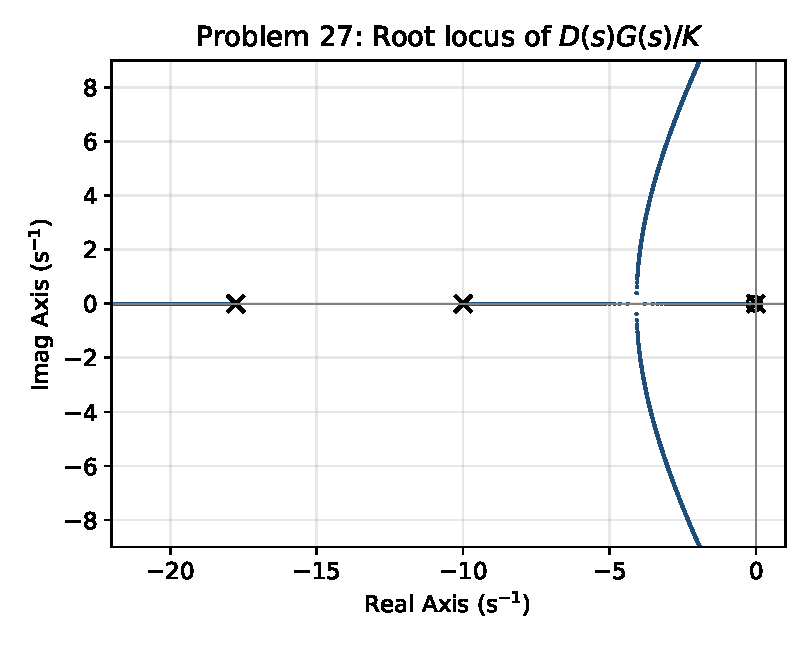
\includegraphics[width=\linewidth]{figures/p27_rlocus.pdf}
  \caption{(d) P27 root locus of the final $D(s)G(s)$.}
  \label{fig:p27rl}
\end{minipage}\hfill
\begin{minipage}{0.49\linewidth}\centering
  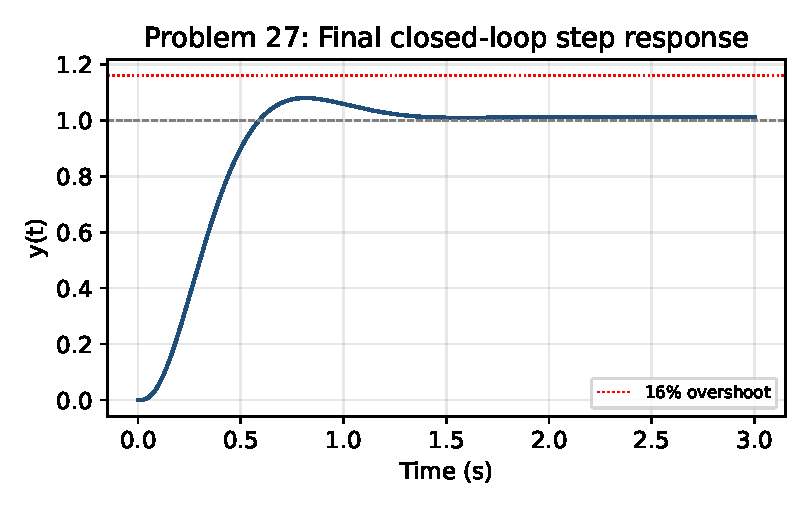
\includegraphics[width=\linewidth]{figures/p27_step.pdf}
  \caption{(e) P27 step response of the final design.}
  \label{fig:p27step}
\end{minipage}
\end{figure}

\begin{figure}[htbp]
\centering
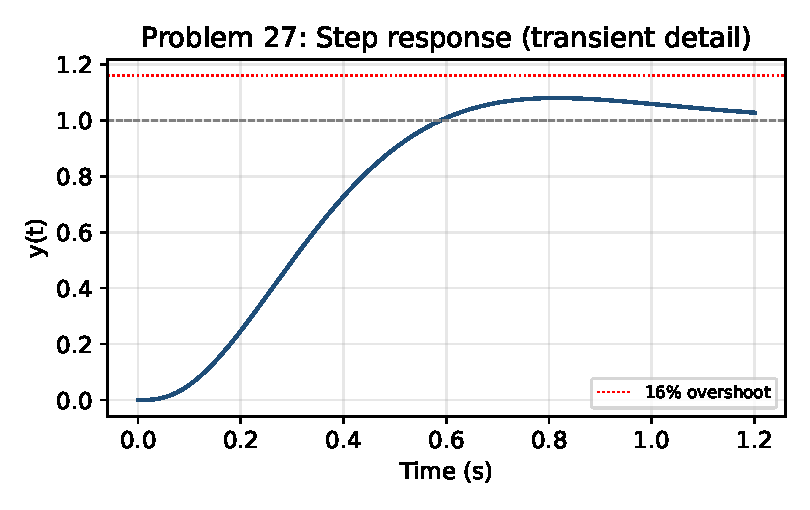
\includegraphics[width=0.55\linewidth]{figures/p27_step_zoom.pdf}
\caption{P27 step response, transient detail: $M_p=7.4\%$ ($<16\%$), $t_r=0.38$~s ($<0.4$~s).}
\label{fig:p27zoom}
\end{figure}

\begin{lstlisting}[style=matlab,caption={Problem 27 --- MATLAB}]
s = tf('s');
G = 10/(s*(s+1)*(s+10));

% --- (a) lead: zeta=0.7, wn=4.5, cancel pole at -1 ---
zeta = 0.65;  wn = 5.5;
s0 = -zeta*wn + 1j*wn*sqrt(1-zeta^2);
ang  = @(z) angle(z)*180/pi;
need = 180 - ang(s0) - ang(s0+10);          % required angle of (s0+p)
p = -real(s0) + imag(s0)/tand(need);         % p = 17.76
K = abs(s0*(s0+p)*(s0+10))/10;               % K = 62.36
Dlead = K*(s+1)/(s+p);

% --- (b) proportional Kv ---  Kv = kp ; kp=50 -> unstable
roots([1 11 10 500])                         % check RHP poles

% --- (c) lag: raise Kv past 50 ---
alpha = 25;  z = 0.05;  plag = z/alpha;
Dlag = (s+z)/(s+plag);
D = Dlead*Dlag;
L = D*G;  T = feedback(L,1);
Kv = dcgain(s*L)                             % ~88  -> ess = 0.011
stepinfo(T)                                  % Mp, tr, ts
figure, rlocus(L)                            % (d)
figure, step(T)                              % (e)
\end{lstlisting}

\FloatBarrier
% ====================================================================
\problem{28}{Lag design for prescribed dominant poles}

\noindent
\[
  G(s)=\frac{1}{s(s+2)} ,
\]
with dominant closed-loop poles at $s=-1\pm j$ and ramp error $e_{ss}<0.2$.

\begin{solution}
\textbf{Gain to meet the transient.} With proportional gain $K$,
$L(s)=\dfrac{K}{s(s+2)}$ and $s^2+2s+K=0$ gives $s=-1\pm\sqrt{1-K}$. The real part is fixed at
$-1$ for every $K$ (the sum of roots is $-2$), so $-1\pm j$ lies \emph{exactly} on the locus
and is obtained with
\[
  1-K=-1\;\Longrightarrow\;K=2 \qquad(\zeta=\tfrac{1}{\sqrt2}=0.707,\ \omega_n=\sqrt2).
\]
No lead is needed. The resulting velocity constant is
$K_v=\lim_{s\to0}sL(s)=K/2=1$, so $e_{ss}=1$ --- far too large.

\medskip
\textbf{Lag compensation.} Add $D_{\text{lag}}(s)=\dfrac{s+z}{s+p}$ with ratio
$\alpha=z/p$. Since $K_v=\frac{K}{2}\,\alpha=\alpha$, the requirement $e_{ss}<0.2$
($K_v>5$) needs $\alpha>5$; take $\alpha=10$ for margin and place the dipole close to the
origin so the dominant poles barely move: $z=0.02$, $p=z/\alpha=0.002$. The compensator is
\[
  \boxed{\,D(s)=\dfrac{2(s+0.02)}{s+0.002}\,},\qquad K_v=10,\qquad e_{ss}=\tfrac{1}{10}=0.1<0.2 .
\]
The lag contributes only $\approx-1^\circ$ at $s_0=-1+j$, so the dominant poles stay at
$\approx-0.99\pm j0.99$ ($\simeq -1\pm j$); the third (lag) pole near $-0.02$ is almost
cancelled by the zero at $-0.02$ and is non-dominant. The step and unit-ramp responses
(Fig.~\ref{fig:p28rl}--\ref{fig:p28ramp}) confirm the dominant pole placement and the reduced
ramp error.
\end{solution}

\begin{figure}[htbp]
\centering
\begin{minipage}{0.49\linewidth}\centering
  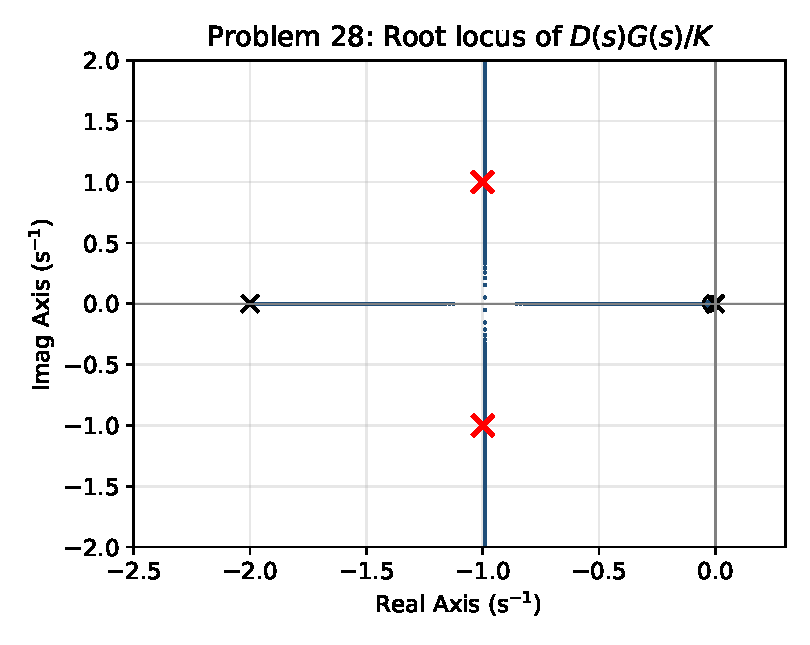
\includegraphics[width=\linewidth]{figures/p28_rlocus.pdf}
  \caption{P28 root locus; $\times$ marks $-1\pm j$.}
  \label{fig:p28rl}
\end{minipage}\hfill
\begin{minipage}{0.49\linewidth}\centering
  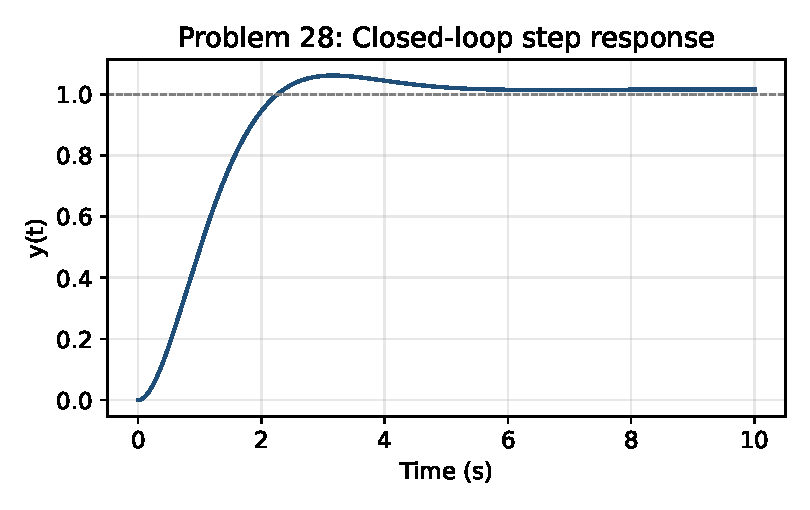
\includegraphics[width=\linewidth]{figures/p28_step.pdf}
  \caption{P28 closed-loop step response.}
  \label{fig:p28step}
\end{minipage}
\end{figure}

\begin{figure}[htbp]
\centering
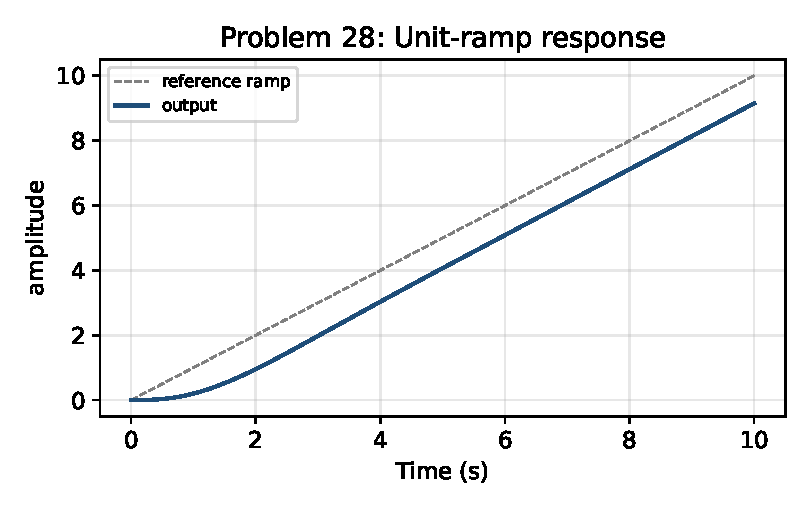
\includegraphics[width=0.55\linewidth]{figures/p28_ramp.pdf}
\caption{P28 unit-ramp response; the steady tracking error settles to $e_{ss}=0.1$.}
\label{fig:p28ramp}
\end{figure}

\begin{lstlisting}[style=matlab,caption={Problem 28 --- MATLAB}]
s = tf('s');
G = 1/(s*(s+2));
K = 2;                       % places poles at -1 +/- j
% lag: alpha = 10 -> Kv = 10, ess = 0.1
z = 0.02;  p = 0.002;
D = K*(s+z)/(s+p);
L = D*G;  T = feedback(L,1);
damp(T)                      % dominant poles ~ -1 +/- j
Kv = dcgain(s*L)            % = 10  -> ess = 0.1
figure, rlocus(L), sgrid
figure, step(T)
t = 0:0.01:10;  figure, lsim(T,t,t)   % unit-ramp response
\end{lstlisting}

\vfill
\begin{center}\small\textcolor{gray}{Designed via root-locus angle/magnitude conditions and verified numerically.}\end{center}

\end{document}
